\section{Optimizing Utility with Variable Hardware}
\label{sec:optimization}

One way to combat increasing power variability is for an application to decrease or increase quality, thereby decreasing or increasing energy consumption.  In this section we explore an architecture for adapting quality when applications have some degree of elasticity---that is, when quality is not a hard constraint.   This will be accomplished by introducing task \emph{knobs}---task-specific expressions of quality and power elasticity. 

\subsection{Task Modeling}
We start first by introducing an application as a set of $N$ {tasks} denoted $\tau_i,~i = 1,\ldots,N$, where each task represents a periodic application subprocess.  We associate with each task and with the application as a whole a utility $u_i$ (or $u_{sys}$ for the entire application) with the understanding that utility represents some notion of quality that the user is interested in. 
While some efforts espouse an architecture wherein each $u_i$ is defined by an arbitrary function (\cite{green2010} for example), we advocate a simplified model where the OS constructs $u_i$ based on a few key inputs from the developer.  In doing so, we assume that $u_i$ is a monotonically non-decreasing function of the active computational time for $\tau_i$ denoted $t_{a,i}$ or, equivalently, the duty cycle ratio specific to $\tau_i$ denoted $d_i$ and defined as $d_i = t_{a,i}/(t_{a,i} + t_{s,i})$ where $t_{s,i}$ is the amount of time that $\tau_i$ is inactive. These variables along with additional key variables used throughout the text are summarized in Table \ref{tab:vars}.\\

\noindent\emph{\underline{Task Knobs}}: 
In order to tune the active time used per task and thus the task-specific duty cycle ratio $d_i$, we introduce the notion of task knobs.  In practical terms, a task knob is a variable that will govern either (1) the period of a task or (2) the frequency with which a task is activated. We argue that a large portion of tasks found in embedded applications will fall in one of these two classes, and those that require both frequency and period modulation can often be divided into two legal subtasks coupled with inter-process communications. For example, tasks that fall under class 1 include variable length sensing tasks, tasks that listen for inbound communication, and variable length processing chains.  Those that fall under class 2 include variable frequency transmission, variable frequency sensor sampling, time synchronization handshaking, control and actuation events, and more.  

We define task knobs, denoted $k_i$, such that increasing $k_i$ will increase $t_{a,i}$, $d_i$, and consequently $u_i$.  Task knobs are created by passing a variable address to the OS, allowing direct manipulation of knob values by an optimization routine.  In addition, the developer specifies a minimum and maximum knob value, $k_{i,min}$ and $k_{i,max}$. The value $k_{i,min}$ specifies the minimum value of $k_i$ that yields a nonzero utility.  Below this value, a task offers no utility.  The value $k_{i,max}$ specifies a value after which increasing $k_i$ further will yield  no added utility.  \\
%As an example, a radio transmission task may be useless if it does not meet a certain latency requirement, but usefulness may plateau at some frequency governed perhaps by the physics and time response of the event being sensed.\\

\noindent\emph{\underline{Generating Utility Curves}}: Changing each knob value $k_i$ will cause a corresponding change in duty cycle ratio $d_i$ based on the nature of $\tau_i$.  Given $k_{i,min}$ and $k_{i,max}$ as well as a mapping from $k_i$ to $d_i$ (to be discussed later) we can construct a utility function $u_i = f(d_i)$ as a modified logistic (Sigmoid) function of the form $f(d_i) = {1\over{1 + e^{-c_id_i}}}, ~c_i \ge 0$.  A logistic function is used because the convex portion of the characteristic \emph{s}-like curve offers a convenient form for modeling diminishing returns on $k_i$.   The convex portion of the logistic function can be isolated by choosing $u_i$ to be of the particular form

\begin{equation}
\label{eq:util}
u_i(d_i) = { 2\over { 1 + e^{-c_id_i }} }- 1, ~~c_i \ge 0, ~~d_{i,min} \le d_i \le d_{i,max}
\end{equation}

where $d_{i,min}$ and $d_{i,max}$ are task duty cycles corresponding to $k_{i,min}$ and $k_{i,max}$.  Here, $c_i$ governs the convergence rate of $u_i$ from the minimum utility to the maximum utility and is calculated as a function of $k_{i,min}$ and $k_{i,max}$ such that 99\% of the utility has been reached by $k_{max}$.  Increasing the percentage of $u_{i,max}$ realized by $k_{i,max}$ has the effect of steepening the utility curve and thus increasing the rate at which returns diminish. The constant $c_i$ can be calculated from Equation \ref{eq:util} by enforcing $u_i(d_{i,max}) - u_i(d_{i,min})$ to be $\epsilon = 0.99$ as shown below:

\begin{equation}
c_i = { -\log\left( {2\over \epsilon + 1} - 1 \right) \over (d_{i,max} - d_{i,min}) }, ~~~~\epsilon = 0.99
\end{equation}

\begin{figure*}[t]
\centering
{\centering
\begin{minipage}{0.47\textwidth}
  \centering

\captionof{table}{\label{tab:vars}Summary of selected variables}
\centering
\begin{tabular}{c|c}
\hline
Variable name & Definition \\ \hline
$\tau_i$ & Task $i,~~i = 1,\ldots,N$ \\
$t_{a,i}$ & Active time for $\tau_i$ \\
$t_{s,i}$ & Inactive time for $\tau_i$ \\
$d_i$ & D.C. ratio for $\tau_i$ \\
$\pmb{d}$ & the vector $[d_1 \cdots d_N]$ \\
$d_{sys}$ & System-wide D.C. \\
$k_i$ & Knob value for $\tau_i$ \\
$\pmb{k}$ & the vector $[k_1 \cdots k_N]$ \\
$\mathcal{K}_i$ & model of $k_i \rightarrow d_i$ \\
$u_i$ & utility fcn. for $\tau_i$ \\
$p_i$ & priority scalar for $\tau_i$ \\
$E$ & energy budget \\
$L$ & desired lifetime \\ \hline
\end{tabular}

\end{minipage}
\hspace{.04\textwidth}
\begin{minipage}{0.47\textwidth}
  \centering
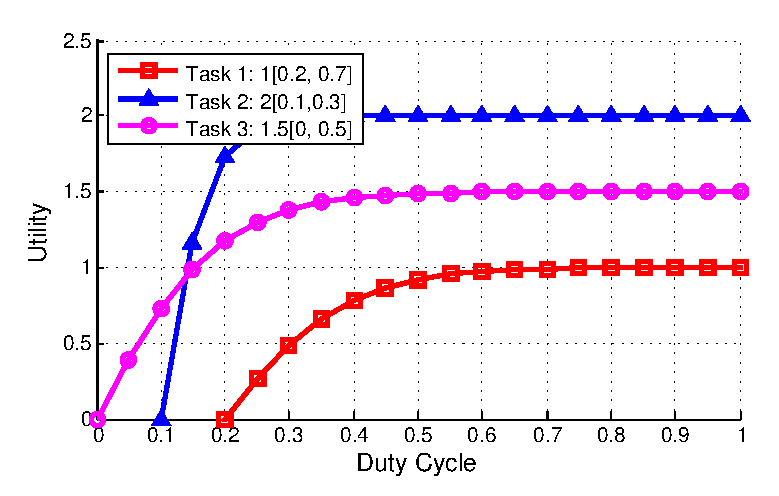
\includegraphics[width=\textwidth]{figures/utilityfunctions}
  \captionof{figure}{\label{fig:util}Example utility curves. Task 1 has priority scalar $p_1 =  1$ with useful range $d_1 = [0.2, 0.7]$, task 2 with $p_2 = 2$ and $d_2 = [0.1, 0.3]$, and finally task 3 with $p_3 = 1.5$ and $d_3 = [0, 0.5]$.}
\end{minipage}
}
\end{figure*}

Finally, each utility curve can be arbitrarily increased or decreased by a priority scalar $p_i \in \R^+$ for tasks with intrinsically higher or lower utility than others.  This offers a level of customizability in addition to specifying $k_{i,min}$ and $k_{i,max}$, allowing the developer to give preference to one task over another. Figure \ref{fig:util} shows three example utility curves corresponding to three tasks with various priorities and duty cycle ranges (resulting from various $k_{i,min}$ and $k_{i,max}$). \\

\noindent\emph{\underline{Learning $\mathcal{K}_i$, the $k_i \rightarrow d_{i}$ Relation}}: Because the developer has free reign to use the knob $k_i$ for each task as desired, the function mapping $k_i$ to active time $t_{a,i}$ and thus $d_i$ is not known \emph{a priori}. Instead, the transformation $\mathcal{K}_i$ that maps $k_i$ to $d_{i}$  is assumed linear and is learned through regression at runtime. Should the developer misuse $k_i$ in a way that is nonlinear or that results in non-increasing values of $t_{a,i}$, the linear model will introduce errors that will affect the optimization process. Dividing active time accumulated per task by a fixed supervisory time interval $t_{super}$ yields task-specific duty cycle ratios, $d_i$. 


\subsection{Maximizing Application Utility}
\label{sec:optimization:maxutil}
Given the set of tasks $\{\tau_1,\ldots, \tau_N\}$, our ultimate goal is to optimize $u_{sys} = \sum_{i=1}^Nu_i$, the overall system utility. That is, we seek a solution to the convex optimization problem

\begin{equation}
\label{eq:linprog_util}
u_{sys}^* = \max_{\pmb{k}} \sum_{i=1}^N{ 2\over { 1 + e^{-c_i\mathcal{K}_i[k_i] }} }- 1,
\end{equation}
\begin{align*}
\text{subject to:~~~~} \sum_{T=T_{min}}^{T_{max}}f_T\mathcal{L}[\pmb{k}] \le { E \over L} = \bar{P} \\ 
\end{align*}

Where $T_{min}$ and $T_{max}$ are the minimum and maximum temperatures for a given location, $\pmb{k} = [k_1 ~\cdots~ k_N]$ is the vector of task knobs, and $\mathcal{L}$  is a linear mapping from $\pmb{k}$ to power consumption.  The parameters $E$ and $L$ are the energy budget and desired lifetime as specified by the user and resulting in an average power goal, $\bar{P}$. In general, $\mathcal{L}$ is a function of temperature, and thus summing over the range of temperatures $[T_{min}~~T_{max}]$ and scaling by the probability density of each temperature $f_T$ gives the predicted power consumption corresponding to the knob vector $\pmb{k}$. When using external peripherals (such as radios, analog to digital converters, and flash storage), $\mathcal{L}$ incorporates both external power and internal power (i.e., power consumed by the processor).  In the remainder of this paper, we will focus on optimizing utility when $\mathcal{L}$ includes the power consumption of the processor alone.  We leave inclusion of peripheral power models as a natural and straightforward extension to the proposed architecture. 

We shift our focus now from that of optimizing utility with a power constraint to that of optimizing utility with a duty cycle constraint.  In other words, power consumption of the system as a whole can take on values in the range $[P_s(T) ~~P_a(T)]$ for a given temperature $T$ dictated by the overall system duty cycle ratio, $d_{sys} = \sum_{i=1}^Nd_i$: $P = (1-d_{sys})P_s + d_{sys}P_a$. Again, both $P_s$ and $P_a$ are functions of temperature so that, replacing $\mathcal{L}$ with the processor power models, the optimization problem becomes

\begin{equation}
\label{eq:linprog_dc}
u_{sys}^* = \max_{\pmb{d}} \sum_{i=1}^N{ 2\over { 1 + e^{-c_id_i }} }- 1,
\end{equation}
\begin{align*}
\text{subject to:~~~~} &\sum_{T=T_{min}}^{T_{max}}f_T\left[\sum_{i=1}^N\left( d_iP_a(T) + (1-d_i)P_s(T)\right)\right] \le {E\over L} = \bar{P} \\ 
\end{align*}

Here we have replaced the knob vector $\pmb{k}$ with the duty cycle vector $\pmb{d}$ similarly defined.  The system-wide duty cycle can be arrived at if we know \emph{a priori} the future environmental temperatures, the function mapping temperature to sleep power $P_s$, and the function mapping temperature to active power $P_a$. Given these, the optimal (maximum)  duty cycle $d_{sys}^* \in [0,1]$ follows naturally from Equation \ref{eq:linprog_dc}: 

\begin{equation}
\label{eq:linprog_fin}
d_{sys}^* = \max ~{d}~~
\end{equation}
\begin{align*}
\text{subject to:~~~~}  \sum_Tf_T\left[dP_a(T) + (1-d)P_s(T)\right] \le {E\over L} = \bar{P}
\end{align*}

%Arriving at $d^*$ is done in the same way as set forth in \cite{Wanner:2012} with the exception that the active and idle/sleep powers ($P_a$ and $P_s$) are learned at runtime.  

Under practical conditions as outlined in \cite{Wanner:2012}, a close approximation for the optimal solution to Equation \ref{eq:linprog_fin} can be obtained algebraically using Equation \ref{eq:dstar}, where we have introduced the temperature-averaged power quantities $\bar{P_s}$ and $\bar{P_a}$:

\begin{equation}
\label{eq:dstar}
d_{sys}^* =  { E - L\bar{P_s} \over L(\bar{P_a} -\bar{P_s}) } 
\end{equation}


\begin{figure*}[t]
\centering
{\centering
\begin{minipage}{0.47\textwidth}
  \centering
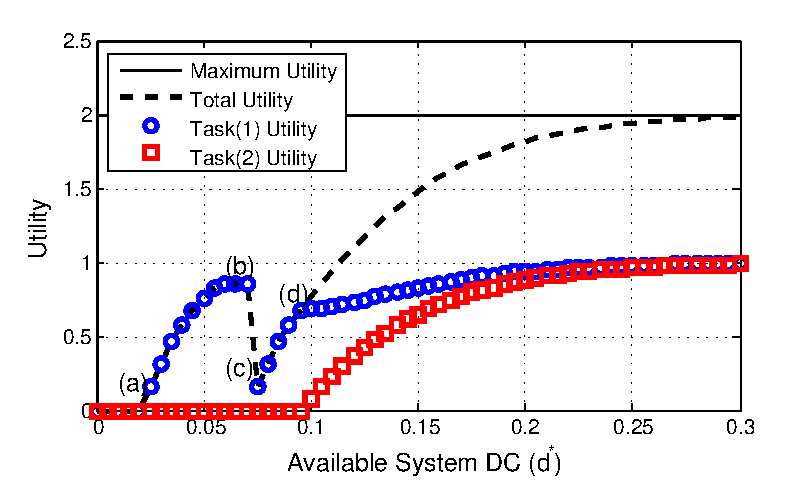
\includegraphics[width=\textwidth]{figures/optimalDCexample}
  \captionof{figure}{\label{fig:optimaldc_mult}Maximizing utility for two tasks and different values of system duty cycle, $d_{sys}^*$}
\end{minipage}
\hspace{.04\textwidth}
\begin{minipage}{0.47\textwidth}
  \centering
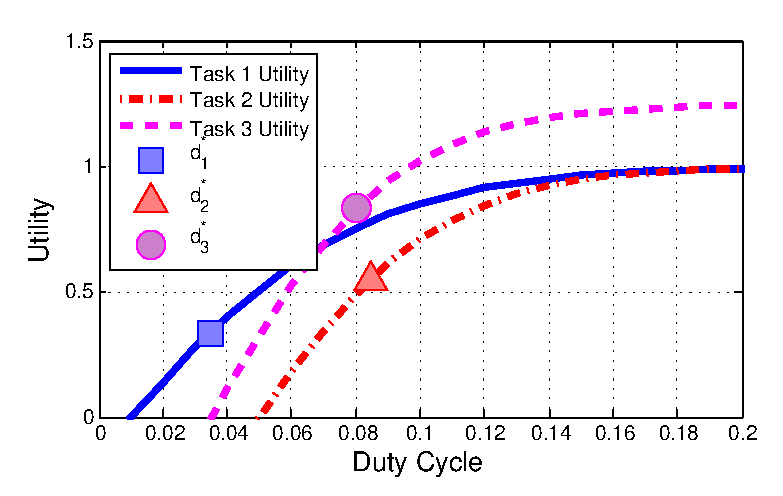
\includegraphics[width=\textwidth]{figures/utilanddc}
  \captionof{figure}{\label{fig:utilanddc}Example optimal duty cycle points for 3 example tasks with different values for $\{k_{min},k_{max}, p_i\}$}
\end{minipage}
}
\end{figure*}

Given $d_{sys}^*$, we now seek an efficient solution to Equation \ref{eq:linprog_dc}.  Because we have chosen $u_i$ to be a logistic function, we can use a greedy approach when optimizing utility.  The optimization routine will be a two step process: (1) attempt to assign the minimum duty cycle $d_{i,min} = \mathcal{K}_i[k_{i,min}]$ needed for each task in order of decreasing priority, and (2) continue distributing computational time in small increments to those tasks yielding the largest marginal utility until no active computational time is left. This process is outlined in Algorithm \ref{alg}. Duty cycle is incrementally added by a small fraction $\delta$ (chosen sufficiently small to ensure accuracy) to those tasks with the largest marginal utility defined as 

\begin{equation}
max\_mu = \max\{mu_1,\ldots,mu_N\},~~~ mu_i = { u_i[d_i+\delta] - u_i[d_i]   \over \delta }
\end{equation}

until $d_{sys}^*$ as calculated from Equation \ref{eq:dstar} is exhausted. Figure \ref{fig:optimaldc_mult} shows an example of the utility maximization algorithm for two example tasks with the total system duty cycle on the $x$-axis and utility on the $y$-axis. .  At point (a), $k_{1,min}$ is met and task 1 begins to receive active time.  At point (b), task 1 begins to plateau as $mu_1$ diminishes.  At point (c), both $k_{1,min}$ and $k_{2,min}$ can be met; starting with task 1 with the highest $mu$, utility is increased until point (d) where task 2 and 1 go back and forth bidding for active time.  The dashed curve illustrates the total system utility, $u_{sys} = u_1 + u_2$. 

% Algorithm
\begin{algorithm}[t]
\SetAlgoNoLine
\KwIn{System duty cycle, $d_{sys}^*$, linear functions $\{\mathcal{K}_1,\ldots,\mathcal{K}_N \}$, and utility curves $\{u_1,\ldots,u_N\}$ }
\KwOut{The optimal task duty cycles $\pmb{d}^* = \{d_1^*,\ldots,d_N^*\}$}
$\pmb{\tau} \leftarrow \text{sort}(\{\tau_1,\ldots,\tau_N\})$ by decreasing $p_i$\\
$d_{remaining} \leftarrow d_{sys}^*$.  \\
//{ Assign minimum knob values for tasks that can be scheduled:}\\
$\pmb{\tau}_{scheduled} \leftarrow \{~\}$ // empty set \\
 \For{$i \in \pmb{\tau}$}{
 	\eIf{$\mathcal{K}_i[k_{i,min}] < d_{remaining}$}{
 	$d_i = \mathcal{K}_i[k_{i,min}]$\\
	$d_{remaining} \leftarrow d_{remaining} - d_i$ \\
	append $\tau_i$ to  $\pmb{\tau}_{scheduled}$
 	}{
 	stop
 	}
 }
 // Allocate remaining duty cycle fairly:\\
 \While{$d_{remaining} > 0$}{
 	// Find highest marginal utility $max\_mu$ and the set $\pmb{\tau}_{max}$ of tasks yielding $max\_mu$:\\
	$[max\_mu, \pmb{\tau}_{max}] \leftarrow$ Find Maximum Marginal Utility$(\pmb{\tau}_{scheduled})$\\
	 $d_{requested} \leftarrow \min\{ \delta \cdot |\pmb{\tau}_{max}|, ~d_{remaining} \}$\\
	 \For{$i \in \pmb{\tau}_{max}$}{
		$d_i \leftarrow d_i + {1\over |\pmb{\tau}_{max}|}d_{requested}$
	 }
 }
$\pmb{d}^* \leftarrow \{d_1,\ldots, d_N\}$
\caption{\label{alg}Greedy Utility Optimization}
\label{alg:one}
\end{algorithm}

Each point in Figure \ref{fig:optimaldc_mult} represents a different environmental set up---that is, a different $d_{sys}^*$ ($x$-axis) resulting from, perhaps, different values for $E$, $L$, and $\pmb{f}_T$. At each $d_{sys}^*$, all tasks are assigned a specific duty cycle ratio $d_i$.  For example, Figure \ref{fig:utilanddc} shows the resulting duty cycles $\{d_1, d_2, d_3\}$ for three tasks when $d_{sys}^* = 0.2$.  The vector $\pmb{d}$ that maximizes Equation \ref{eq:linprog_dc} is denoted $\pmb{d}^* = \{d_1^*,\ldots,d_N^*\}$. 

With a method in hand to calculate an optimal $d_{sys}^*$ offline, we seek a method for both calculating $d_{sys}^*$ and achieving $d_i \in \{d_1,\ldots,d_N\}$ in an efficient, online manner.  Our implementation of this architecture is called VaRTOS and is the subject of the following section. 



